\bookchapter{Exact spin sources and finite thermal structure}
\label{ch:spin-foundation}

\subsection{What the spin construction contributes to matter}

The spin program supplies a family of finite interacting sources with a complete account of their states. Its contribution to matter construction starts at that level. A specified source has an interaction, an energy convention, retained boundary coordinates, a preparation and a receiving observable. Complete spectra and thermal factors then calculate how internal states contribute to a finite response. The later nuclear constructions receive this method through their actual contact phases and source actions. Their connection is established by those maps, rather than by counting every binary coordinate as an additional material constituent.

This dedicated section develops the completed spin work in five steps. The present chapter defines the exact sources and their thermal organization. Chapter~\ref{ch:spin-microscopic} follows a specified microscopic source through hidden memory and ordered readings. Chapter~\ref{ch:spin-composition} develops composition control and its kinetic response. Chapter~\ref{ch:spin-physical} brings the complete physical response bounds through the latest source Dirichlet result. Chapter~\ref{ch:spin-connections} maps the resulting objects into the surrounding volumes. The organization is editorial synthesis; each source result retains its original model, numerical scope and classification.\samref{SPF_SYNTHESIS}

The distinction between sources matters from the beginning. The dense signed packet systems, the Kac-normalized composition sources, the all-temperature hidden-spin compiler and the actual isotope phase encodings have different Hamiltonians and clocks. They share exact counting, conditional preparation and retained-history methods. The section states which source is acting before using its results.

\subsection{The full energy, magnetization and boundary measure}

For binary coordinates $s_i\in\{-1,+1\}$, the source convention is
\begin{equation}
 E(s)=-\sum_{i<j}J_{ij}s_i s_j-\sum_i h_i s_i,
 \qquad M(s)=\sum_i s_i.
\end{equation}
Four ordered ports carry a boundary address $b\in\{0,\ldots,15\}$. The exact joint density is
\begin{equation}
 g(E,M,b)=\#\{s:E(s)=E,\ M(s)=M,\ B(s)=b\}.
\end{equation}
The complete counting identities are
\begin{equation}
 \sum_{E,M,b}g(E,M,b)=2^N,
 \qquad \sum_{E,M}g(E,M,b)=2^{N-4}.
\end{equation}
A stored nonzero coefficient represents all assignments with its energy, magnetization and boundary. The number of stored coefficients and the number of source states therefore have different roles. The joint measure retains their exact relationship.\samref{SPF_N2000}

The completed six-case $N=2000$ calculation contains 244,104,392 nonzero primary records. Every source has 1,999,000 nonzero pair interactions and all sixteen boundary assignments. Three deterministic parent families are each completed with uniform fill $J_0=+1$ or $-1$. The packet/$+1$ member is the ferromagnetic analytic control; the other five members contain frustrated cycles. The six-case set consequently keeps a useful unfrustrated comparator within the same exact counting construction.

The parent consists of 133 fifteen-spin packets and one five-spin terminal packet. A full packet has three complete five-spin layers and two interlayer perfect matchings. The signed variant reverses a selected edge in each layer. The chain variant adds alternating-sign gateway bridges. The complete fill acts on every missing pair; it is an actual term in the energy, including when its correction representation is sparse.

Write $\Delta J_{ij}=J_{ij}-J_0$. Since $M^2=N+2\sum_{i<j}s_i s_j$, the energy separates exactly as
\begin{align}
 E&=E_c-\frac{J_0}{2}(M^2-N),\\
 E_c&=-\sum_{i<j}\Delta J_{ij}s_i s_j-\sum_i h_i s_i.
\end{align}
The uniform dense interaction is retained through $M$; the correction graph supplies the local factors. This is why magnetization must survive the contraction. A correction energy marginal alone would discard its association with the dense energy.

For correction bound $\mathcal B=\sum|\Delta J_{ij}|+\sum|h_i|$, define $k=(M+N)/2$ and $t=(E_c+\mathcal B)/2$. The source emits exact coefficients in $(k,t,b)$ and reconstructs
\begin{equation}
 M=2k-N,\qquad
 E=2t-\mathcal B-\frac{J_0}{2}\big[(2k-N)^2-N\big].
\end{equation}
Local packet polynomials and signed gateway contractions evaluate this full measure. In the recorded production, separately computed global encodings agree for all 96 case/boundary tables. The large integer state counts remain available for subsequent field, temperature and boundary queries.\samref{SPF_N2000}

The shared installation extends that retained object into exact response queries. It preserves scalar energy densities and ordered boundary rows while adding joint $E,M,b$ solving, rational fields, fixed-magnetization queries, moments and covariance. Its actual adoptions include the retained ATOM3D six-spin sources and Starbreaker's N100 source. This is a completed computational connection between the matter inputs and Volume III's exact-state machinery.\samref{SPF_INSTALL}

\subsection{Thermal preparation retains the source normalization}

The joint counts give a boundary partition sum
\begin{equation}
 Z_b(\beta,h)=\sum_{E,M}g(E,M,b)e^{-\beta(E-hM)}.
\end{equation}
Their ratios supply boundary preparations; their derivatives supply energy and magnetization response. An absolute free energy retains its normalizing prefactor. A common factor can cancel in a ratio without disappearing from the complete source ledger.

The early large thermal ladder and the later transition program use different normalizations. For the archived positive-fill source,
\begin{equation}
 H_N=-\frac{M^2-N}{2}+C_N,
 \qquad \beta_N=\frac{c_N}{N},\qquad
 c_N=1+\frac{\lambda}{\sqrt N}.
\end{equation}
This scales the entire Hamiltonian by $1/N$, including its sparse correction. If the correction has $L=O(N)$ negative edges, $|C_N|\leq2L$ gives, for fixed bounded $c>0$,
\begin{equation}
 \left|\frac{\log Z_N-\log Z_N^{(0)}}N\right|
 \leq\frac{2cL}{N^2}.
\end{equation}
The pressure per spin approaches the uniform-source result in this normalization while finite boundary weights continue to carry the actual correction. The completed compact thermal ladder reaches $N=10^{57}+10$ with its specified source factors. That compact evaluation retains a full normalized source; it does not materialize a graph or an expanded joint table of that size.\samref{SPF_THERMAL}

The phase-transition and composition family instead fixes sparse strength:
\begin{equation}
 \mathcal H_N=-\frac{M^2-N}{2N}+\kappa C_N,
 \qquad \kappa\geq0,
\end{equation}
at inverse temperature of order one. The dense fill has Kac strength $1/N$, while each sparse component retains order-one correction strength. A spin called free in this construction has no sparse negative edge; it still participates in the dense interaction.

For positive dense coupling, Gaussian decoupling gives the full boundary integral
\begin{equation}
 Z_b=\mathcal C_N\int_{\mathbb R}e^{-Ny^2/(2\beta)}
 L_{\mathrm{root},b}(y)\prod_jL_j(y)^{n_j}\,dy.
\end{equation}
The local factors contain their actual couplings and multiplicities. The finite root retains its ordered ports. The directed consumer pays local series remainders, finite-factor errors, origin panels and infinite tails. Algebraic cancellation of the large quadratic pieces improves accuracy without dropping any part of the complete integral. This construction supplies the finite preparations used in the subsequent memory and composition studies.\samref{SPF_SYNTHESIS}\samref{SPF_TRANSITION}

\subsection{From ordinary onset to controlled higher-order criticality}

For repeated-component magnetization response $m_0(y)$ and susceptibility $\chi=m_0'(0)$, the retained packet sources satisfy
\begin{equation}
 m_0(y)<\chi y\quad(y>0),\qquad
 \beta_c\chi(\beta_c,\kappa)=1.
\end{equation}
The exact global response certificate excludes an earlier distant ordered maximum. At the first onset, global uniqueness and a negative quartic stabilizer give continuous ordering. The earlier stronger global-concavity route has two retained counterexamples; the completed transition statement uses response domination. The source therefore preserves the successful mathematical argument and the useful failed route together.\samref{SPF_TRANSITION}

The critical points respond to the actual component content. At $\kappa=1$, the signed-packet and chain thresholds are approximately 1.663814710634 and 1.663815941534. Their susceptibility difference is
\begin{equation}
 \chi_{\rm chain}-\chi_{\rm signed}
 =-\frac{a(1-a)^2}{15},\qquad a=\tanh(2\beta\kappa),
\end{equation}
so the chain threshold lies higher for every finite positive correction strength. These are source-specific ordering statements, with the original boundary retained.

\begin{figure*}[tbp]\centering
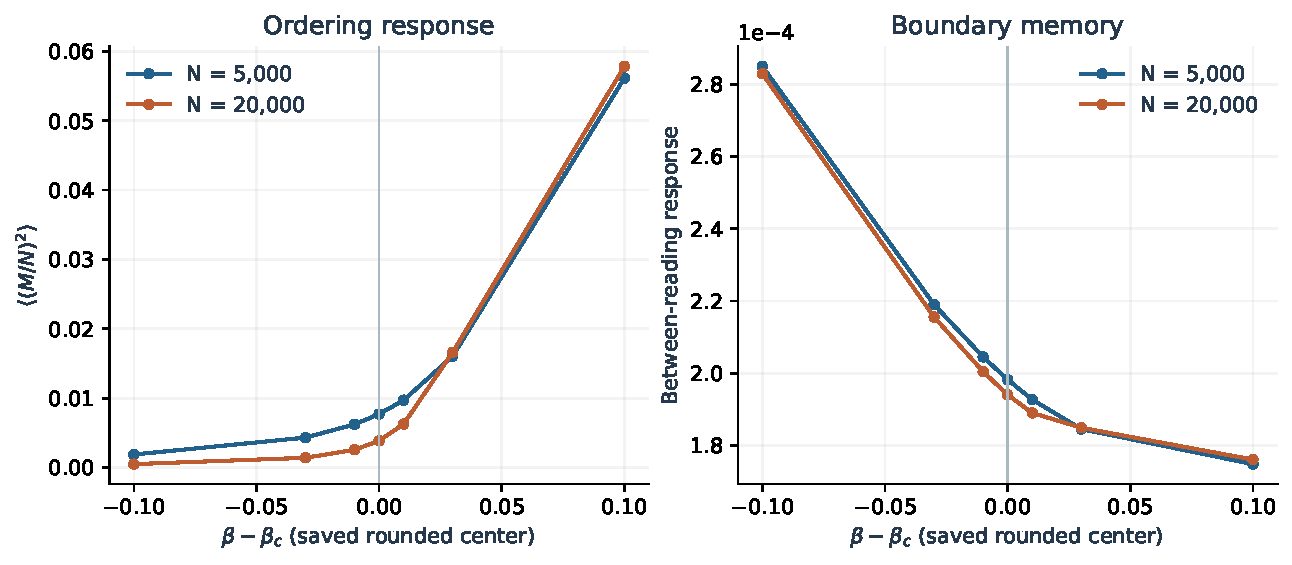
\includegraphics[width=\textwidth]{figures/transition_memory.pdf}
\caption{Recorded chain-source ordering and between-reading memory near the saved rounded critical center at $\kappa=1$. The two panels use the same finite sources and different observables. Lines connect retained data; this edition performs no thermal recalculation.\samref{SPF_FIG_TRANSITION}}
\label{fig:spin-transition}
\end{figure*}

Varying the correction-free fraction gives exact tricritical members:
\begin{table*}[tbp]\centering\small
\begin{tabular}{lccc}\toprule
Bulk components & Free fraction & $\beta_t$ & $\kappa_t$\\\midrule
Negative pairs & $1/5$ & $5/3$ & $3\log3/20$\\
Four-spin path plus four pairs & $77/461$ & $461/261$ & $261\log3/1844$\\\bottomrule
\end{tabular}
\end{table*}
Their negative sixth cumulants supply the stabilizer after the quartic term vanishes. At the displayed fixed couplings, fractions above the critical fraction have continuous first onset, and sufficiently close fractions below it have first-order onset. Critical squared magnetization scales as $N^{-1/3}$. The recorded pair control with a vanishing quartic term and a positive sixth term shows why the quartic zero alone does not classify the transition. The ratio result carries the classification: \emph{The test result suggests strong contact with the concept.}\samref{SPF_RATIO}

Negative triangles add an odd frustrated cycle as a different local component. The pure triangle/free family has an ordinary continuous first transition for every allowed free fraction and $\kappa\geq0$, with a positive quartic stabilizer. Mixing pairs, triangles and correction-free spins gives a different exact point:
\begin{align}
 \nu&=\frac9{20},&\tau&=\frac{343}{640},&f&=\frac9{640},\\
 \beta_c&=\frac{32}{15},&\kappa&=\frac{15\log3}{128}.
\end{align}
A 1920-spin bulk cell contains 432 pairs, 343 triangles and 27 correction-free spins. The fifteen-spin root and five-spin tail remain, so $N=20+1920r$. The quadratic, quartic and sextic pressure coefficients vanish, leaving
\begin{equation}
 \Phi_c(y)=-C_8y^8+O(y^{10}),\qquad C_8=\frac3{3584}.
\end{equation}
The source has a global all-field certificate as well as this local expansion. The leading stabilizer is eighth order; its boundary response need not be an eighth derivative.\samref{SPF_TRIANGLE}

With $\xi=C_8^{1/8}N^{1/8}y$, the normalized limiting density is
\begin{equation}
 p_u(\xi)\propto\exp(u\xi^2-\xi^8).
\end{equation}
The field scale is $N^{-1/8}$, the leading squared-magnetization and boundary-memory scale is $N^{-1/4}$, and the temperature window is $N^{-3/4}$. The finite calculation retains the root, tail, exact reference and physical Gaussian correction. In the completed first-correction panel, 85 of 90 observable comparisons improve; the five lower-size exceptions remain part of the result. The directed comparisons evaluate complete finite sources rather than treating the truncated local polynomial as a global Hamiltonian.\samref{SPF_OCTIC}

\begin{figure*}[tbp]\centering
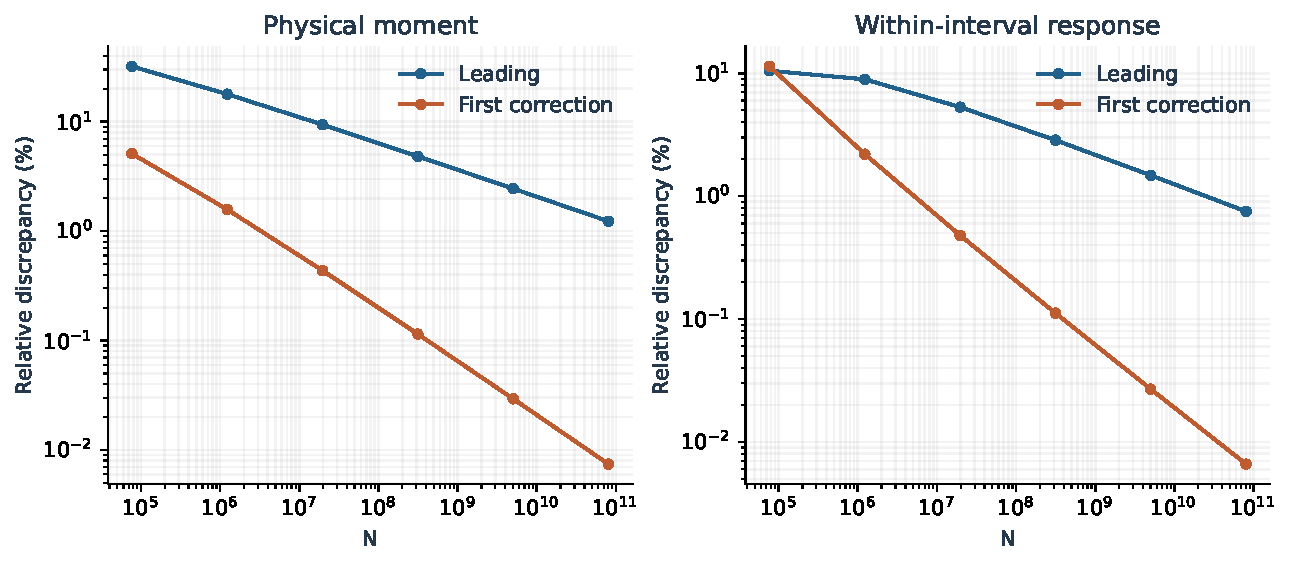
\includegraphics[width=\textwidth]{figures/octic_corrections.pdf}
\caption{Saved $u=0$ comparisons of the eighth-order leading and first-correction rules for the physical moment and within-interval response. These selected curves retain their original finite values; the complete source panel and its five lower-size exceptions have the scope stated in the text.\samref{SPF_FIG_OCTIC}}
\label{fig:spin-octic}
\end{figure*}

\subsection{A finite crossover preserves actual controls and boundary histories}

Temperature and pair/triangle fractions provide three independent physical source controls near the mixed point. In $x=\tanh^2y$, the completed control Jacobian has rank three and determinant $25/351232$. The local unfolding law is
\begin{equation}
 p(\xi)\propto\exp(\alpha\xi^2+\lambda\xi^4+\sigma\xi^6-\xi^8).
\end{equation}
The exact inverse control construction and global derivative bounds retain the associated finite source. The named dimensionless control coordinates are not the physical coupling constants of the later isotope or continuum receiver.\samref{SPF_UNFOLD}

The uniform crossover joins the eighth-order origin to merging ordered endpoints. Its simple limiting form is
\begin{equation}
 p_s(z)\propto e^{-(z^2-s)^4}.
\end{equation}
Changing variable to $t=z^2-s$ retains its half-line support and Jacobian:
\begin{equation}
 p(t)\propto\mathbf1_{t>-s}(s+t)^{-1/2}
 \exp(vt+rt^2+dt^3-g t^4),\qquad g>0.
\end{equation}
Both field endpoints and the actual rounded integer component counts enter the complete consumer. The source theorem supplies a second thermal remainder of order $N^{-3/4}$ and pressure remainder of order $N^{-7/4}$ in its stated neighborhood. All 126 first and 63 second comparison improvements pass in the selected completed crossover panel. Three reused endpoint integrals retain their earlier identities.\samref{SPF_CROSSOVER}

This thermal organization is already tied to memory. At the chain's exact $\kappa=1$ critical point, the unchanged protocol gives limiting preparation, between-reading and within-interval contributions approximately
\begin{equation}
\begin{gathered}
-0.430454602216,\\
0.000189921648477,\\
0.000344266087525.
\end{gathered}
\end{equation}
The first is a signed preparation contrast, comparing the specified state-zero start with conditional equilibrium inside its initial coarse class. The latter is not a globally stationary initial mixture. All three retain their actual middle relay, accepted state and declared heat-bath interval. Thus a bulk ordering law and a finite boundary history are measurable functions of the same source while answering different questions.\samref{SPF_TRANSITION}

\subsection{What passes to the microscopic and matter constructions}

The completed object consists of a source action, state multiplicities, ordered ports, thermal factors, finite preparation and recorded response. The exact density can answer many future weighted questions; a directed compact consumer answers a selected question using the full factor definition. The next chapters preserve that distinction when they introduce a physical generator, hidden memory and source-conditioned resolvent bounds.

For matter, this provides a constructive route from an admitted finite inventory to an interacting state. The actual Li6 phase map later in this volume retains every source constant and all contact addresses. Its conditional thermal factors carry the hidden-state normalization. The nuclear, atomic and molecular recipients then keep their actual free systems and energy payments. The underlying principle is already visible in the spin source: a complete state space can be evaluated through structured factors while its retained boundary still carries information about what happened before the next contact.

For Volume III, the same structure identifies the executable handoff. Exact integer coefficients, source-bound local factors, conditional traces, matrix intervals and retained operands are different outputs with their own useful scopes. The computation chapter of this section will connect these directly to the shared solver, native operation recipes and recorded recovery. The scientific inputs are the completed constructions developed here; this edition adds their exposition and cross-volume organization.\samref{SPF_INSTALL}
